\documentclass[conference]{IEEEtran}

% =========================
% Packages
% =========================
\usepackage{cite}
\usepackage{url}
\usepackage{amsmath,amssymb,amsfonts}
\usepackage{algorithm}
\usepackage{algorithmic}
\usepackage{graphicx}
\usepackage{textcomp}
\usepackage{xcolor}
\usepackage{array}
\usepackage{makecell}
\usepackage{booktabs}
\usepackage{multirow}
\usepackage{subcaption}
\usepackage[hidelinks]{hyperref}
\usepackage{balance}

\def\BibTeX{{\rm B\kern-.05em{\sc i\kern-.025em b}\kern-.08em
    T\kern-.1667em\lower.7ex\hbox{E}\kern-.125emX}}

% =========================
% Title / Authors
% =========================
\title{From Dwell Potential to Planning Districts: A Three-Stage
       Framework for Urban EV Fast-Charging Planning}

\author{
\IEEEauthorblockN{Ehsan Sobhani}
\IEEEauthorblockA{
  Department of Electrical Engineering and Computer Science\\
  York University, Toronto, Canada\\
  ehsan666@yorku.ca}
\and
\IEEEauthorblockN{Hany E.\,Z. Farag}
\IEEEauthorblockA{
  Department of Electrical Engineering and Computer Science\\
  York University, Toronto, Canada\\
  hefarag@yorku.ca}
}

\begin{document}
\maketitle

% =========================
% Abstract
% =========================
\begin{abstract}
Urban EV fast-charging planning requires identifying locations where
vehicles naturally dwell long enough to charge and organizing these
locations into stable meso-scale planning regions.
This paper introduces a three-stage behavioral-to-structural framework
applied to 234 arterial zones in Toronto, Canada.
Stage~1 constructs an \emph{Activity-Based Dwell Potential} (ABDP)
metric from point-of-interest (POI) categories weighted by a Gaussian
dwell-time compatibility kernel centred at $T^*=30$\,min.
Stage~2 proposes \emph{Neutralization-Based Zonal Clustering} (NBZC),
a shape-constrained, contiguity-preserving greedy algorithm that
compresses the 234-zone rook-adjacency graph into 107 meso-scale
clusters whose internal ABDP--BEV imbalance is approximately neutralized.
A full-factorial sensitivity sweep over 1\,008 configurations selects the
Pareto-knee operating point ($|\texttt{max}|=8$ zones,
$\lambda_{\mathrm{shape}}=0.001$, $r_{\max}=2000$\,m).
Stage~3 detects planning districts from the 107-node cluster graph via
an exhaustive community-detection sweep of 2\,296 candidate partitions,
using a two-stage knee--Pareto--stability model-selection procedure.
The selected partition yields $k^*=24$ planning districts with
neutralization objective $J=0.2808$, modularity $Q=0.449$,
coverage $0.494$, performance $0.964$, and aggregate stability
$S=0.956$, demonstrating that behavioral self-sufficiency and
structural cohesion emerge jointly from the proposed framework.
\end{abstract}

\begin{IEEEkeywords}
EV fast charging, activity-based dwell potential, spatial regionalization,
neutralization clustering, community detection, corridor planning
\end{IEEEkeywords}

% =========================
% I. Introduction
% =========================
\section{Introduction}

Fast-charging (FC) deployment requires spatial units that align with
how charging opportunities arise: vehicles charge while parked, and
parking durations are driven by nearby activities.
Mobility-only indicators (traffic flow, BEV density) capture where
vehicles move but do not encode where vehicles \emph{dwell} long enough
to fast charge. Conversely, fine spatial units exhibit strong local
mismatch between BEV density and dwell compatibility, leading to
fragmented and unstable planning decisions.

This paper proposes a three-stage framework:
\begin{enumerate}[label=(\roman*)]
  \item A behavioral signal layer: \emph{Activity-Based Dwell Potential}
        (ABDP), a dwell-time-weighted POI density normalized to $[0,1]$.
  \item A regionalization layer: \emph{Neutralization-Based Zonal
        Clustering} (NBZC), which forms contiguous, compact corridor
        regions that approximately neutralize BEV--ABDP imbalance.
  \item A district-selection layer: an exhaustive community-detection
        sweep combined with a two-stage knee--Pareto--stability criterion
        to select the final number of planning districts.
\end{enumerate}

\subsection{Contributions}
\begin{itemize}
  \item A dwell-compatible ABDP metric that reframes POIs as behavioral
        feasibility signals aligned with fast-charging session durations.
  \item NBZC: a shape-constrained, contiguity-preserving clustering
        algorithm with a Pareto-knee parameter-selection procedure over
        1\,008 full-factorial configurations.
  \item A two-stage knee--Pareto--stability community-detection
        framework that selects $k^*=24$ planning districts from
        2\,296 candidate partitions.
  \item Empirical validation on 234 Toronto arterial zones demonstrating
        simultaneous improvement in behavioral neutralization and graph
        structural cohesion.
\end{itemize}

% =========================
% II. Literature Review
% =========================
\section{Literature Review}

\subsection{Evolution of EV Charging Infrastructure Planning}
Early EV infrastructure research treated demand as an exogenous,
spatially aggregated variable derived from traffic volumes, population
density, or vehicle ownership statistics \cite{BIAN2022}.
Recent studies have transitioned toward user-centric paradigms that
incorporate trajectory data, land-use characteristics, and
socio-economic indicators to improve spatial responsiveness to demand.
However, most models still infer charging needs from mobility intensity
rather than activity-specific behavioral dynamics.

\subsection{POI-Based Demand Modeling}
POI data have been widely used to classify functional urban zones and
identify charging hotspots via kernel density estimation, $k$-means,
DBSCAN, location entropy, and geographic weighted regression.
Empirical evidence shows strong correlations between certain POI
categories and charging station distribution \cite{Zechao2024}.
However, POIs are predominantly treated as static demand intensifiers
rather than behavioral anchors, leaving the temporal dimension of dwell
duration compatibility with fast charging largely unmodeled.

\subsection{Graph-Based and ML Approaches}
Support vector regression, multi-view graph convolutional networks, and
topology-informed graph models have improved predictive performance for
charging demand \cite{Wang2023}.
Multi-objective optimization frameworks including evolutionary algorithms
and deep reinforcement learning balance cost, coverage, and fairness
objectives \cite{Sun2024}.
Despite these advances, behavioral feasibility—alignment between natural
dwell time and required charging duration—is typically abstracted away.

\subsection{Research Gap}
A fundamental gap persists: the absence of a meso-scale planning framework
that quantitatively integrates activity-driven dwell compatibility into
endogenous regionalization.
The present work addresses this gap by embedding behavioral feasibility
directly into the regionalization objective through ABDP and NBZC,
and by coupling the result with a systematic community-detection sweep to
derive planning districts.

% =========================
% III. Data and Notation
% =========================
\section{Data and Notation}

\subsection{Urban Arterial Zones and Study Area}
The study area consists of $N_{\mathrm{Ar}}=234$ arterial zones covering
the Toronto urban corridor network, projected to UTM zone~17N
(EPSG:32617) so that all distance computations are in metres.
Each zone $Z^{\mathrm{Ar}}_j$ is a planar polygon with area
$A^{\mathrm{Ar}}_j>0$.

\subsection{Normalized BEV Density}
Let $\rho^{\mathrm{Ar}}_j = EVC^{\mathrm{Ar}}_j / A^{\mathrm{Ar}}_j$
be the areal EV density.
Normalized BEV density is
\begin{equation}
S^{\mathrm{EV}}_j =
\frac{\rho^{\mathrm{Ar}}_j - \min_k \rho^{\mathrm{Ar}}_k}
     {\max_k \rho^{\mathrm{Ar}}_k - \min_k \rho^{\mathrm{Ar}}_k}
\;\in[0,1].
\end{equation}

\subsection{POI Assignment}
Each POI $p$ is assigned to its containing zone via
$\phi(p)=j$ if $\mathbf{x}_p\in Z^{\mathrm{Ar}}_j$,
giving the count $N_{jk}$ of POIs of category $k$ in zone $j$.

\subsection{Rook-Contiguity Graph}
Spatial adjacency is encoded as
$G=(V,E)$, $|V|=234$, $|E|=502$,
with one connected component.
An edge $(i,k)\in E$ exists iff zones $i$ and $k$ share a boundary
segment of positive length under rook contiguity.

% =========================
% IV. Activity-Based Dwell Potential (ABDP)
% =========================
\section{Activity-Based Dwell Potential (ABDP)}

\subsection{Dwell-Time Compatibility Weight}
Fast charging is behaviorally viable when vehicle dwell duration
approximates the charging session length.
Let $T^*=30$\,min be the target duration and $\sigma=10$\,min the
tolerance width.
The Gaussian dwell-compatibility weight for POI category~$k$ is
\begin{equation}
w_k =
\exp\!\left(-\frac{(T_k - T^*)^2}{2\sigma^2}\right).
\label{eq:w_k}
\end{equation}
Table~\ref{tab:dwell_weights} reports the eight POI categories and their
weights under these parameters.

\begin{table}[t]
\centering
\caption{POI Dwell Times and Compatibility Weights ($T^*=30$\,min,
         $\sigma=10$\,min)}
\label{tab:dwell_weights}
\small
\begin{tabular}{lcc}
\toprule
Category & $T_k$ (min) & $w_k$ \\
\midrule
Food service & 30 & 1.000 \\
Healthcare   & 40 & 0.607 \\
Retail       & 45 & 0.287 \\
Services     & 20 & 0.607 \\
Leisure      & 60 & 0.014 \\
Education    & 90 & $<$0.001 \\
Transit      & 10 & 0.135 \\
Office       & 120 & $<$0.001 \\
\bottomrule
\end{tabular}
\end{table}

\subsection{Zone-Level ABDP}
The weighted POI mass for zone $j$ is
\begin{equation}
S^{\mathrm{act}}_j = \sum_{k\in\mathcal{K}} w_k\, N_{jk}.
\end{equation}
Area-normalized dwell density:
\begin{equation}
D_j = S^{\mathrm{act}}_j \,/\, A^{\mathrm{Ar}}_j.
\end{equation}
Min-max normalization yields the ABDP score
\begin{equation}
\bar{D}_j =
\frac{D_j - \min_k D_k}{\max_k D_k - \min_k D_k}
\;\in[0,1].
\end{equation}

% =========================
% V. From Behavioral Signal to Meso-Scale Regionalization
% =========================
\section{From Behavioral Signal to Meso-Scale Regionalization}

The zone-level imbalance
\begin{equation}
d_i = \bar{D}_i - S_i^{\mathrm{EV}}
\end{equation}
measures directional mismatch between dwell compatibility and EV
concentration.
At fine spatial resolution, these imbalances are highly volatile:
the mean zone-level neutralization index
$\bar{\eta}_i = 0.422$ and the median is $0.385$
(Table~\ref{tab:neutralisation}), indicating that a typical arterial
zone is far from internally balanced.

Planning decisions based exclusively on either signal introduce
systematic bias.
Neutralization addresses this tension by aggregating adjacent zones
with opposing imbalances so that positive and negative deviations
offset at the cluster level, producing regions where
$\bigl|\sum_{i\in C} d_i\bigr|\approx 0$.

% =========================
% VI. NBZC Algorithm
% =========================
\section{Neutralization-Based Zonal Clustering (NBZC)}

\subsection{Compactness Proxy}
Let $\mathbf{x}_i\in\mathbb{R}^2$ be the centroid of zone $i$.
The cluster radius is
\begin{equation}
r(C) = \max_{i\in C}\|\mathbf{x}_i - \bar{\mathbf{x}}_C\|,
\quad
\bar{\mathbf{x}}_C = \frac{1}{|C|}\sum_{i\in C}\mathbf{x}_i.
\end{equation}

\subsection{Combined Score}
\begin{equation}
\mathrm{score}(C\cup\{j\}) =
\Bigl|\sum_{i\in C\cup\{j\}} d_i\Bigr|
+ \lambda_{\mathrm{shape}}\,r(C\cup\{j\}).
\label{eq:score}
\end{equation}

\subsection{Greedy Frontier Growth and Stopping Rules}
Clusters grow by seeding from $\arg\max_{i\in U}|d_i|$ and
iteratively absorbing the rook-adjacent unassigned zone that minimizes
\eqref{eq:score}.
Growth halts when:
\begin{itemize}
  \item $|C|\ge\texttt{max\_cluster\_size}$;
  \item adding the best candidate would violate
        $\mathrm{imb}>\texttt{max\_abs\_imbalance}$;
  \item candidate radius exceeds $\texttt{max\_radius\_m}$;
  \item imbalance worsens for $|C|\ge2$.
\end{itemize}

\begin{algorithm}[t]
\caption{NBZC: Greedy Neutralization + Shape-Constrained Clustering}
\label{alg:nbzc}
\begin{algorithmic}[1]
\STATE \textbf{Input:} $G=(V,E)$, $\{d_i\}$, $\{\mathbf{x}_i\}$,
       $\lambda$, $s_{\max}$, $b_{\max}$, $r_{\max}$
\STATE $U \leftarrow V$, $\mathcal{C}\leftarrow \emptyset$
\WHILE{$U\neq\emptyset$}
  \STATE $i^*\leftarrow\arg\max_{i\in U}|d_i|$;
         $C\leftarrow\{i^*\}$; $U\leftarrow U\setminus\{i^*\}$
  \WHILE{true}
    \STATE $F\leftarrow\bigl(\bigcup_{i\in C}N(i)\bigr)\cap U$
    \IF{$F=\emptyset$} \STATE \textbf{break} \ENDIF
    \STATE $j^*\leftarrow\arg\min_{j\in F}\mathrm{score}(C\cup\{j\})$
    \IF{any stopping rule fires} \STATE \textbf{break} \ENDIF
    \STATE $C\leftarrow C\cup\{j^*\}$; $U\leftarrow U\setminus\{j^*\}$
  \ENDWHILE
  \STATE $\mathcal{C}\leftarrow\mathcal{C}\cup\{C\}$
\ENDWHILE
\STATE \textbf{Output:} $\mathcal{C}$
\end{algorithmic}
\end{algorithm}

% =========================
% VII. Evaluation Metrics
% =========================
\section{Evaluation Metrics}
\label{sec:eval_metrics}

\subsection{Cluster-Level Neutralization Index}
For cluster $c$:
\begin{equation}
\Delta_c = \sum_{i\in c} d_i, \qquad
\eta_c =
\frac{|\Delta_c|}{\sum_{i\in c}(\bar{D}_i + S_i^{\mathrm{EV}})}.
\label{eq:eta_c}
\end{equation}
Zone-level baseline: $\eta_i = |d_i|/(\bar{D}_i+S_i^{\mathrm{EV}}+\epsilon)$.

\subsection{Community-Level Neutralization Objective}
For community $g$ in the cluster graph:
\begin{align}
\Delta_g &= \textstyle\sum_{c\in g} d_c, \quad
T_g = \textstyle\sum_{c\in g}(\bar{D}_c+S_c^{\mathrm{EV}}), \\
\eta_g   &= |\Delta_g|/T_g, \\
J(k)     &= \textstyle\sum_g \eta_g T_g \,/\, \textstyle\sum_g T_g.
\label{eq:J}
\end{align}
Lower $J$ indicates stronger behavioral self-sufficiency.

\subsection{Structural Quality}
Coverage (fraction of intra-community edges), modularity $Q$, and
performance (fraction of correctly classified node pairs) as defined in
\cite{nx_comm}.

% =========================
% VIII. Results
% =========================
\section{Results}

\subsection{Zone Graph}
The rook-contiguity graph over 234 arterial zones has 502 edges and
forms a single connected component.
Structural summary: mean degree 4.29, transitivity 0.1882, average
local clustering 0.1905, average shortest path 7.44, diameter 18,
radius 11 (Table~\ref{tab:graph_metrics}).

\subsection{Sensitivity Analysis and Parameter Selection}

A full-factorial sensitivity sweep was conducted over
$6\times7\times4\times6=1\,008$ NBZC configurations.
Parameter ranges:
\begin{itemize}
  \item $\texttt{max\_cluster\_size} \in \{2,4,8,12,15,20\}$,
  \item $\texttt{max\_abs\_imbalance} \in \{0.1,0.2,0.3,0.5,0.7,0.8,1.0\}$,
  \item $\lambda_{\mathrm{shape}} \in \{0,0.0002,0.0005,0.001\}$,
  \item $r_{\max} \in \{\infty,1000,2000,4000,6000,8000\}$\,m.
\end{itemize}
Each run was evaluated on two minimization objectives:
total absolute cluster imbalance $\sum_c|\eta_c|$ and
mean cluster radius.
Fig.~\ref{fig:pareto_tradeoff} shows the resulting trade-off space.
The Pareto-knee operating point is selected by minimizing the
Euclidean distance to the ideal origin in the normalized objective plane.

\textbf{Selected configuration:}
\begin{center}
\small
\begin{tabular}{ll}
\toprule
Parameter & Value \\
\midrule
$\texttt{max\_cluster\_size}$  & 8 zones \\
$\texttt{max\_abs\_imbalance}$ & 0.5 \\
$\lambda_{\mathrm{shape}}$     & 0.001 \\
$r_{\max}$                     & 2\,000\,m \\
\midrule
Clusters produced ($n_c$)           & 107 \\
$\sum_c|\eta_c|$ (neutralization loss) & 38.82 \\
Mean cluster radius                 & 693\,m \\
\bottomrule
\end{tabular}
\end{center}

\begin{figure}[t]
\centering
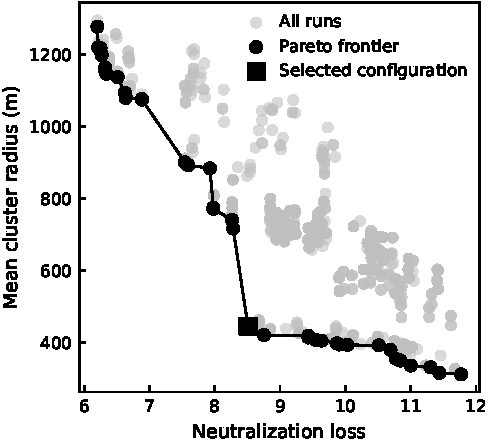
\includegraphics[width=\linewidth]{neutralization_vs_compactness_rook.pdf}
\caption{Neutralization--compactness trade-off across all 1\,008
sensitivity configurations. The Pareto frontier (blue) and selected
knee point (red star) are highlighted.}
\label{fig:pareto_tradeoff}
\end{figure}

\subsection{Neutralization Improvement}

Table~\ref{tab:neutralisation} compares the distribution of the
neutralization index $\eta$ before and after clustering under the
selected configuration.
Aggregation into 107 meso-scale clusters consistently reduces imbalance:
mean $\eta$ falls from 0.422 (zone) to 0.363 (cluster), a relative
improvement of 14.0\%, while the median drops more substantially from
0.385 to 0.288 (25.2\% reduction).
This indicates broad-based improvement across the distribution rather
than correction of a few extreme zones.
The near-zero minimum at the cluster level (0.001) confirms that some
clusters achieve virtually complete internal compensation.
The maximum imbalance is effectively unchanged (1.000 vs.\ 0.999),
indicating that the most extreme structural mismatches require larger
regions to neutralize, consistent with the hard size cap of eight zones.

\begin{table}[t]
\centering
\caption{Zone-Level vs.\ Cluster-Level Neutralization ($\eta$)}
\label{tab:neutralisation}
\small
\begin{tabular}{lcc}
\toprule
Metric & Zone $\eta_i$ & Cluster $\eta_c$ \\
\midrule
Mean   & 0.422 & 0.363 \\
Median & 0.385 & 0.288 \\
Min    & 0.001 & 0.001 \\
Max    & 1.000 & 0.999 \\
\bottomrule
\end{tabular}
\end{table}

\begin{figure*}[t]
\centering
\begin{subfigure}[t]{0.49\textwidth}
  \centering
  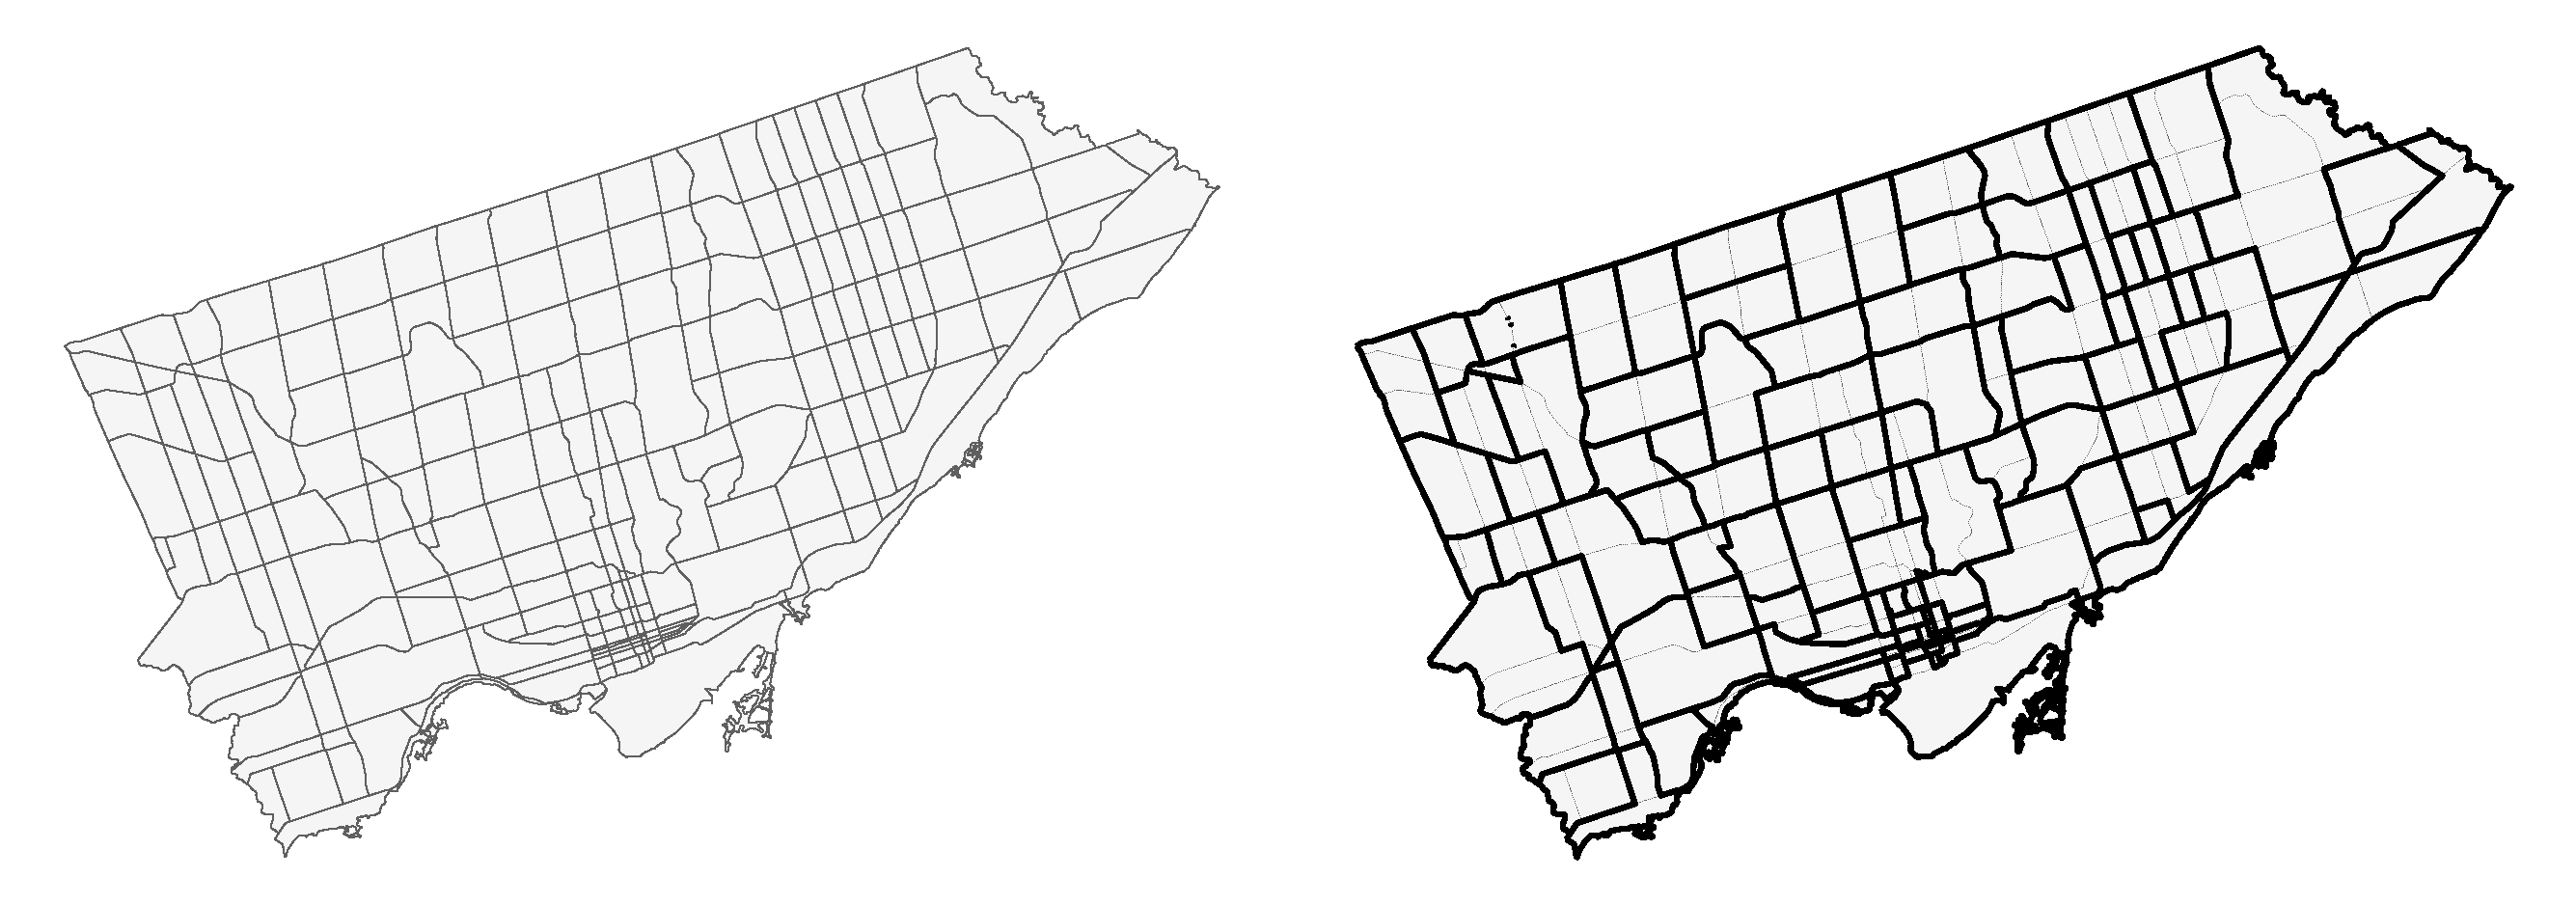
\includegraphics[width=\linewidth]{before_after_clustering.pdf}
  \caption{Before (zone-level imbalance $d_i$) and after (NBZC
           cluster regions) spatial maps.}
  \label{fig:maps}
\end{subfigure}
\hfill
\begin{subfigure}[t]{0.49\textwidth}
  \centering
  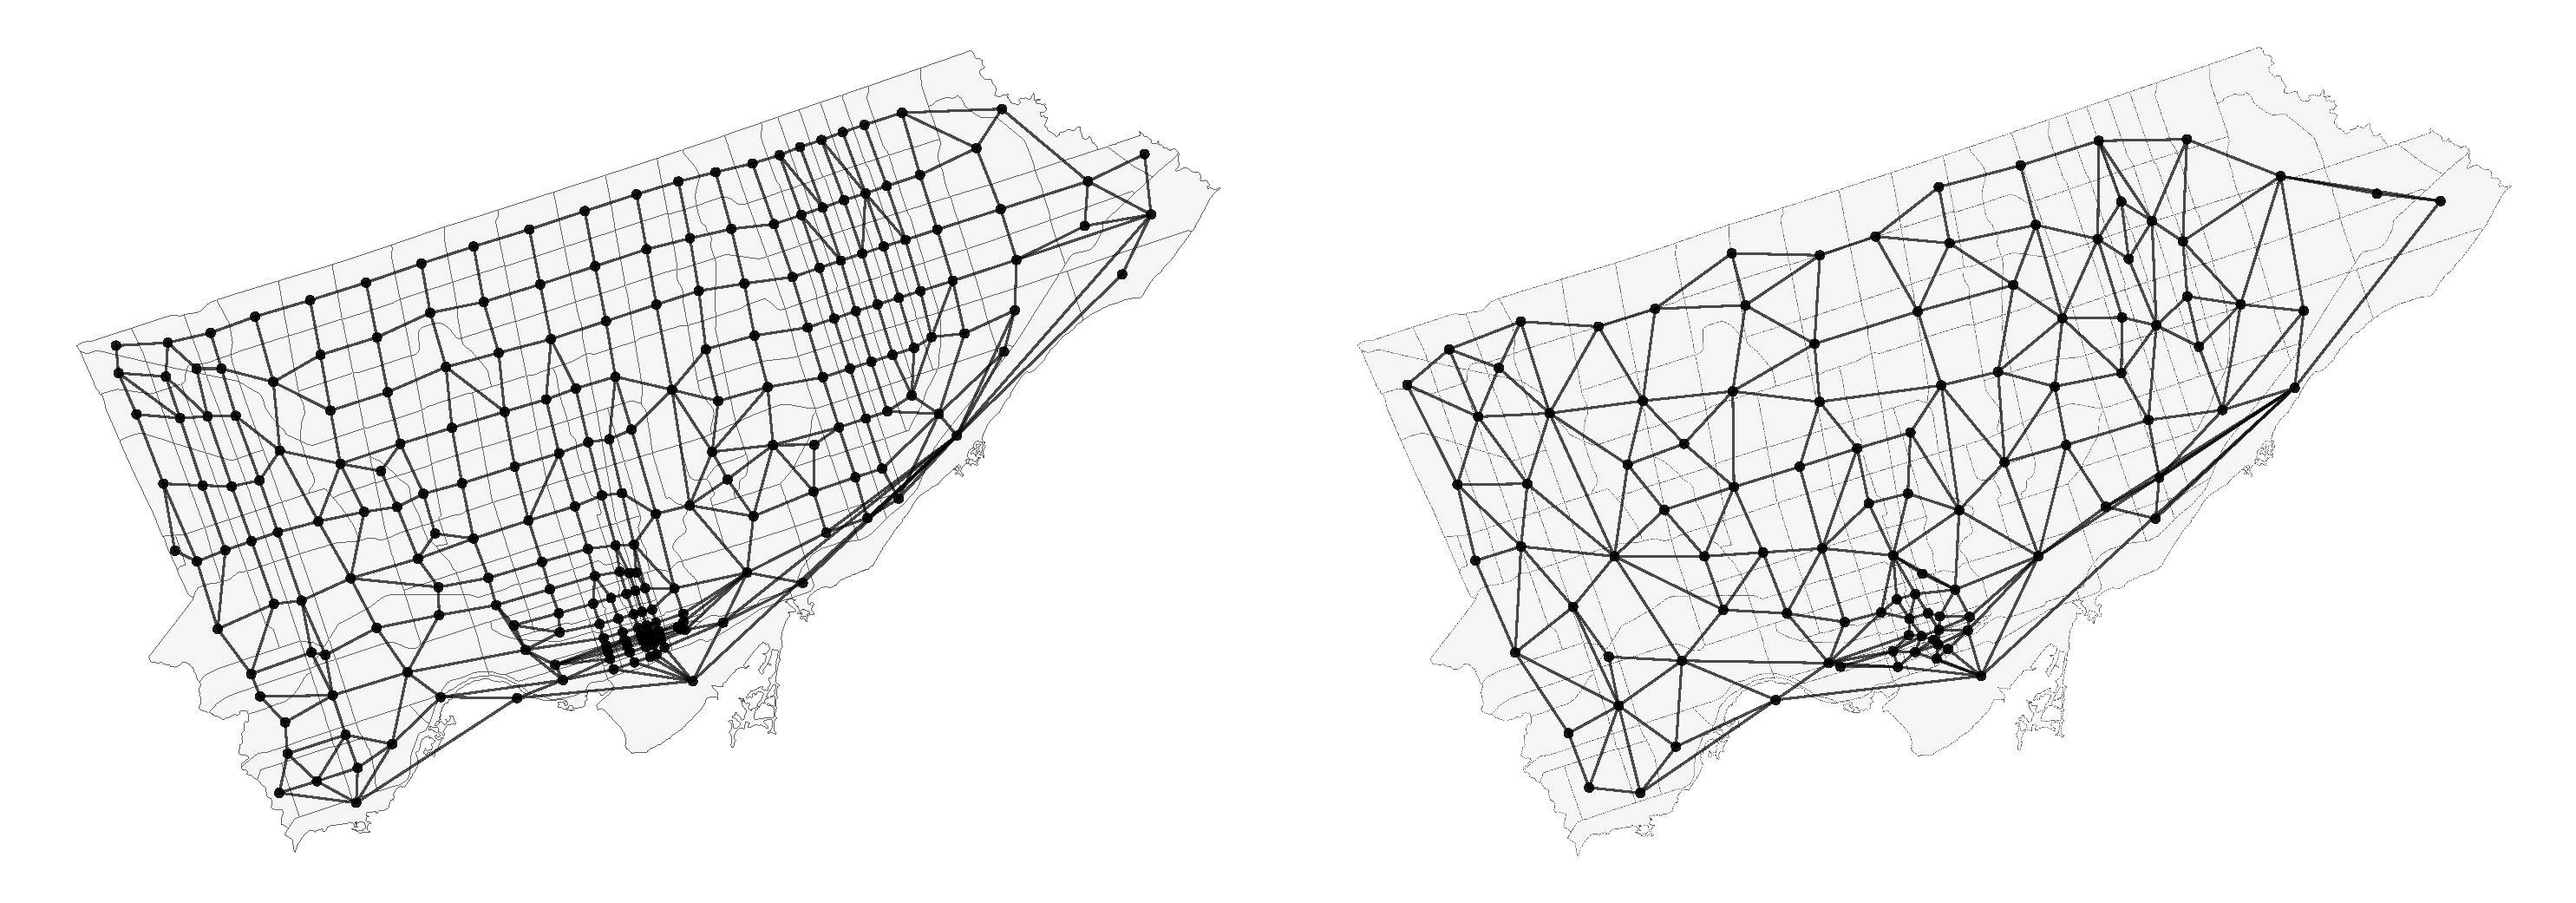
\includegraphics[width=\linewidth]{before_after_graph_comparison.pdf}
  \caption{Zone-level (left) and cluster-level (right) adjacency
           graphs.}
  \label{fig:graphs}
\end{subfigure}
\caption{Spatial and topological transformation induced by NBZC.}
\label{fig:before_after}
\end{figure*}

\subsection{Topological Effects of Regionalization}

Table~\ref{tab:graph_metrics} compares structural graph properties
before and after NBZC.
The zone graph (234 nodes, 502 edges) is compressed to a cluster graph
with 107 nodes and 267 edges while maintaining a single connected
component and zero bridges and articulation points.

Graph cohesion increases substantially.
Density more than doubles (0.0184 $\to$ 0.0471).
Transitivity rises from 0.1882 to 0.3428, and average local clustering
from 0.1905 to 0.423.
The triangle count grows from 112 to 137 despite the 54\% reduction in
node count, confirming stronger local interconnectedness at the
meso-scale.
Navigability improves concurrently: average shortest path falls from
7.44 to 4.62, diameter from 18 to 10, and radius from 11 to 7.
Degree assortativity shifts from mildly positive (0.0717) to mildly
negative ($-0.0675$), indicating that clustering moderates degree
homophily and produces a more balanced inter-regional connectivity
pattern.
The maximum $k$-core is preserved at 3 in both graphs, while the
$k_{\max}$-core size decreases from 230 to 105, reflecting a condensed
but structurally equivalent hierarchical backbone.

\begin{table}[t]
\centering
\caption{Graph Metrics: Zone Graph vs.\ Cluster Graph}
\label{tab:graph_metrics}
\scriptsize
\begin{tabular}{lrr}
\toprule
Metric & Zone graph & Cluster graph \\
\midrule
Nodes ($|V|$)             & 234     & 107 \\
Edges ($|E|$)             & 502     & 267 \\
Density                   & 0.0184  & 0.0471 \\
Components                & 1       & 1 \\
Deg min / med / mean / max & 2/4/4.29/11 & 2/5/4.99/11 \\
Leaf fraction             & 0.000   & 0.000 \\
Transitivity              & 0.1882  & 0.3428 \\
Avg local clustering      & 0.1905  & 0.4230 \\
Triangles (total)         & 112     & 137 \\
Bridges                   & 0       & 0 \\
Articulation points       & 0       & 0 \\
Max $k$-core              & 3       & 3 \\
$k_{\max}$-core size      & 230     & 105 \\
Avg shortest path         & 7.44    & 4.62 \\
Diameter / Radius         & 18 / 11 & 10 / 7 \\
Degree assortativity      & 0.0717  & $-0.0675$ \\
\bottomrule
\end{tabular}
\end{table}

\subsection{Stage 3: Community Detection Sweep}

\subsubsection{Experimental Design}
Six community-detection algorithms were applied to the 107-node cluster
graph:
greedy modularity, label propagation, asynchronous fluid communities
($k\in[2,107]$, 20 seeds), Kernighan--Lin bisection (20 seeds),
Louvain \cite{Blondel2008} ($\gamma\in\{0.3,0.5,0.7,1.0,1.5,2.0\}$, 20 seeds), and
Girvan--Newman (15 levels).
In total, 2\,296 candidate partitions were generated and evaluated on
both $J(k)$ (behavioral) and the structural triple
$\{Q, \mathrm{Coverage}, \mathrm{Performance}\}$.

\subsubsection{Knee Detection}
For each $k$, the best-achievable neutralization is
\begin{equation}
J_{\mathrm{best}}(k) = \min_{\mathcal{G}:|\mathcal{G}|=k} J(\mathcal{G}).
\end{equation}
Fig.~\ref{fig:J_vs_k} shows the resulting curve.
A curvature-based knee is detected at $k_{\mathrm{knee}}=35$, marking
the transition from a rapidly degrading regime (coarse $k$) to a slowly
increasing stable regime.
The admissible scale window is therefore
$\mathcal{K}_{\mathrm{adm}}=\{2,3,\dots,35\}$.

\begin{figure}[t]
\centering
\includegraphics[width=\linewidth]{communities_and_neutralization_knee_curve.pdf}
\caption{$J_{\mathrm{best}}(k)$ curve. The knee at $k_{\mathrm{knee}}=35$
bounds the admissible search space; the final selection $k^*=24$ is
indicated by the dash-dot line.}
\label{fig:J_vs_k}
\end{figure}

\subsubsection{Pareto and Stability Selection}
Within $\mathcal{K}_{\mathrm{adm}}$, the objective vector
\begin{equation}
\mathbf{f}(k) =
\bigl(-J_{\mathrm{best}}(k),\;Q(k),\;\mathrm{Cov}(k),\;\mathrm{Perf}(k)\bigr)
\end{equation}
is maximized jointly.
27 of the 34 admissible $k$ values are Pareto-efficient:
$\mathcal{K}_{\mathrm{Pareto}} = \{2,3,4,5,6,7,8,9,11,12,13,14,15,16,$
$17,18,19,20,21,23,24,25,26,28,29,30,33\}$.

The aggregate stability score
$S(k)=\frac{1}{4}(S_J+S_Q+S_P+S_C)$
is computed over $\mathcal{K}_{\mathrm{Pareto}}$.
The final resolution is
\begin{equation}
k^* = \arg\max_{k\in\mathcal{K}_{\mathrm{Pareto}}} S(k) = 24.
\end{equation}

\subsubsection{Final Partition}
The selected partition uses the \emph{asynchronous fluid communities}
algorithm.
Table~\ref{tab:final_partition} summarizes its metrics.

\begin{table}[t]
\centering
\caption{Final Planning District Partition ($k^*=24$)}
\label{tab:final_partition}
\small
\begin{tabular}{lc}
\toprule
Metric & Value \\
\midrule
Number of districts $k^*$ & 24 \\
Algorithm & Fluid communities \\
Neutralization $J$         & 0.2808 \\
Modularity $Q$             & 0.4490 \\
Coverage                   & 0.4944 \\
Performance                & 0.9639 \\
Aggregate stability $S$    & 0.9556 \\
\bottomrule
\end{tabular}
\end{table}

Table~\ref{tab:admissible_k} lists the admissible-set metrics for
selected values of $k$ around the chosen resolution.

\begin{table}[t]
\centering
\caption{Admissible-Set Metrics for Selected $k$ Values}
\label{tab:admissible_k}
\scriptsize
\begin{tabular}{rcccccc}
\toprule
$k$ & $J_{\mathrm{best}}$ & $Q$ & Coverage & Perf. & Alg. & $S$ \\
\midrule
 2 & 0.1995 & 0.4098 & 0.9101 & 0.543 & KL      & 0.281 \\
 6 & 0.2229 & 0.5867 & 0.7640 & 0.856 & Fluid   & 0.790 \\
12 & 0.2530 & 0.5548 & 0.6442 & 0.932 & Fluid   & 0.864 \\
19 & 0.2588 & 0.4779 & 0.5356 & 0.956 & Fluid   & 0.952 \\
\textbf{24} & \textbf{0.2808} & \textbf{0.4490} & \textbf{0.4944} & \textbf{0.964} & \textbf{Fluid} & \textbf{0.956} \\
30 & 0.2795 & 0.4098 & 0.4494 & 0.967 & Fluid   & 0.856 \\
35 & 0.2960 & 0.3534 & 0.3858 & 0.966 & Fluid   & 1.000 \\
\bottomrule
\end{tabular}
\end{table}

% =========================
% VIII-F. Baseline Comparison
% =========================
\subsection{Baseline Comparison}
\label{sec:baseline}

To verify that the neutralization improvement is attributable to the
NBZC objective rather than to contiguity enforcement or spatial grouping
alone, NBZC is compared against three reference methods on the same
234-zone graph (Table~\ref{tab:baseline}).
All methods that require a target cluster count use $k=107$, equal to
the number produced by NBZC, so that differences in mean metrics are
not confounded by resolution.

\textbf{Spatial KMeans} \cite{MacQueen1967} partitions zones by
Euclidean centroid proximity with no contiguity constraint, representing
the simplest geographic grouping.
\textbf{Random Contiguous} grows $k=107$ connected regions from random
seeds via graph-Voronoi BFS \cite{Erwig2000}, respecting contiguity but
optimising nothing; it provides the key control that isolates the
contribution of the NBZC objective from the contribution of contiguity
alone.

\begin{table}[t]
\centering
\caption{Baseline Comparison ($k=107$; $\downarrow$ lower is better;
         best in bold)}
\label{tab:baseline}
\scriptsize
\setlength{\tabcolsep}{4pt}
\begin{tabular}{lrrrrr}
\toprule
Method & $k$ & $\bar{\eta}_c$\,$\downarrow$ & Med\,$\eta_c$\,$\downarrow$ & Max\,$\eta_c$\,$\downarrow$ & Radius\,(m)\,$\downarrow$ \\
\midrule
\textbf{NBZC (proposed)} & \textbf{107} & \textbf{0.363} & \textbf{0.288} & \textbf{0.999} & \textbf{693} \\
Spatial KMeans \cite{MacQueen1967} & 107 & 0.424 & 0.438 & 1.000 & 508 \\
Random Contiguous \cite{Erwig2000} & 107 & 0.376 & 0.341 & 1.000 & 832 \\
\bottomrule
\end{tabular}
\end{table}

Two findings stand out.
First, NBZC achieves lower $\bar{\eta}_c$ than both KMeans (0.363 vs.\
0.424, a 14.4\% relative reduction) and Random Contiguous (0.363
vs.\ 0.376, a 3.6\% reduction).
Since Random Contiguous enforces the same contiguity constraint as NBZC
but applies no neutralization objective, this 3.6\% gap directly
quantifies the contribution of the NBZC scoring function; the remaining
improvement over KMeans reflects the joint effect of contiguity and the
objective.
Second, KMeans reduces the mean cluster radius to 508\,m (vs.\ 693\,m
for NBZC) by unconstrained geometric partitioning, but yields a 16.9\%
higher $\bar{\eta}_c$, demonstrating that compactness alone does not
serve the neutralization objective.

% =========================
% IX. Discussion
% =========================
\section{Discussion}

\subsection{Behavioral Neutralization}
NBZC achieves a consistent reduction in behavioral imbalance across all
distributional moments (Table~\ref{tab:neutralisation}).
The mean neutralization index falls 14.0\% and the median 25.2\%,
reflecting broad-based improvement rather than correction of extreme
outliers.
The shape constraint ($\lambda_{\mathrm{shape}}=0.001$,
$r_{\max}=2000$\,m) keeps the mean cluster radius at 693\,m, well within
corridor-planning norms, while still achieving substantial neutralization.
The strict size cap of eight zones prevents large meso-regions that
would improve imbalance arithmetically but lose spatial coherence.

\subsection{Structural Consolidation}
Although node count is cut by 54\% (234 $\to$ 107), the cluster graph
gains in nearly every structural quality dimension
(Table~\ref{tab:graph_metrics}).
The doubling of density (0.0184 $\to$ 0.0471) and the increase in
transitivity and local clustering indicate that clusters form denser,
more cohesive corridor-scale regions rather than loosely connected
chains.
The average shortest path falls from 7.44 to 4.62 (38\% reduction),
and the diameter shrinks from 18 to 10.
This confirms that aggregation both simplifies and tightens the
spatial backbone.
The absence of bridges and articulation points in both graphs confirms
that NBZC does not introduce structural fragility.

\subsection{District Resolution Selection}
The two-stage procedure prevents the knee ($k_{\mathrm{knee}}=35$) from
being adopted directly as the district count.
Instead, the knee bounds the admissible window, and Pareto efficiency
combined with stability selects $k^*=24$.
At $k=24$, the fluid partition achieves $J=0.2808$ with $S=0.956$—a
near-maximum stability value within the Pareto set—indicating that small
perturbations to the district count produce minimal behavioral or
structural disruption.
Higher $k$ values (e.g., $k=35$) achieve slightly better stability
($S=1.000$) but at the cost of substantially higher neutralization loss
($J=0.296$) and lower modularity ($Q=0.353$), reflecting excessive
fragmentation.
Coarser resolutions (e.g., $k=6$) offer lower $J$ but yield coverage
of only 0.764 and stability of 0.790, implying over-aggregation that
masks intra-urban heterogeneity.
The selected $k^*=24$ therefore represents the joint optimum across
behavioral, structural, and stability objectives.

\subsection{Contribution Isolation via Baseline Comparison}
Table~\ref{tab:baseline} enables a clean decomposition of the NBZC
improvement.
The Random Contiguous baseline holds contiguity constant while removing
the objective: its $\bar{\eta}_c=0.376$ exceeds the NBZC value of
0.363, confirming that the neutralization scoring function accounts for
the primary portion of the observed improvement and cannot be explained
by contiguity enforcement alone.
Spatial KMeans removes both contiguity and the behavioral signal and
yields the highest $\bar{\eta}_c$ (0.424), demonstrating that geometric
proximity without a behavioral objective provides the weakest
neutralization even when the cluster count is controlled.
NBZC achieves the best neutralization at a planning-relevant spatial
scale ($r=693$\,m, $k=107$), confirming that the frontier-growth
algorithm forms more coherent behavioral regions than either
unconstrained or objective-free alternatives.

\subsection{Planning Implications}
The 24-district partition is directly actionable.
Each district is a contiguous, compact, and behaviorally self-balanced
region of arterial zones within which both EV density and dwell
compatibility are jointly supported.
Unlike externally imposed TAZ-based or administrative boundaries,
these districts emerge endogenously from the interaction between
mobility intensity (BEV density) and behavioral feasibility (ABDP),
making them structurally grounded for downstream capacity allocation
and grid-aware optimization.

% =========================
% X. Conclusion
% =========================
\section{Conclusion}

This paper presented a three-stage behavioral-to-structural framework
for urban EV fast-charging planning, validated on 234 Toronto arterial
zones.
Stage~1 (ABDP) converted POI composition into a dwell-compatible
behavioral signal.
Stage~2 (NBZC) compressed the 234-zone graph into 107 meso-scale
clusters with 14.0\% mean and 25.2\% median reductions in neutralization
index, while simultaneously doubling graph density, increasing
transitivity from 0.19 to 0.34, and reducing average shortest path
from 7.44 to 4.62.
Stage~3 identified 24 planning districts from 2\,296 candidate
partitions via a two-stage knee--Pareto--stability procedure, achieving
$J=0.281$, $Q=0.449$, coverage 0.494, performance 0.964, and aggregate
stability 0.956.

The results confirm that behavioral self-sufficiency and structural
cohesion improve jointly through the proposed cascade.
Future work will integrate the 24-district partition into downstream
capacity allocation and grid-aware optimization, and will evaluate
robustness under temporal variation in activity patterns and EV adoption
trajectories.
\cite{Annan2024}\cite{Katontoka2025}\cite{Zhang2025}\cite{Wang2023}%
\cite{Sun2024}\cite{Matkovic2024}\cite{Qin2026}\cite{Yuan2025}%
\cite{WANG_DENG_YAN_LI_2025}\cite{Zechao2024}\cite{BIAN2022}

% =========================
% References
% =========================
\bibliographystyle{IEEEtran}
\bibliography{references}

\end{document}
